\section{Evaluation}
\label{s:evaluation}
In this section, we address two primary questions: 1. how can downstream feedback be used to to improve prediction accuracy under cost constraints, and 2. how can scheduling policies at the key-level granularity be configured to maximize downstream accuracy? 
\sarah{Joey: State the things that we actually want to show}

To do so, we structure our evaluation in the following way: 
\begin{enumerate}
    \item We construct two workloads (anomaly detection and information retrieval) using real-world data where model predictions rely on pre-computed features that need to be updated as new events are streamed in. 
    \item We run simulation experiments with baseline and configured policies to observe cost/accuracy tradeoffs. 
    We use simulation to more directly evaluate the polices independent of implementation details.
    \item We implement the time-series decomposition workload in \system{} to evaluate performance of baseline versus configured feature maintenance policies in a real streaming setting. 
\end{enumerate}

%We evaluate policies in simulation and system experiments in terms of both resource cost and downstream prediction accuracy. The simulators are used to explored cost and accuracy tradeoffs for scheduling policies with different configurations, which are used to identify improved \textit{policy parameters} which specify key-level scheduling policies. These parameters can be fed back into the simulator or into real streaming systems to improve performance on later data. 

%A machine learning pipeline using a feature store has both a featurization system, which maintains feature values, as well as a model serving system, which queries feature values. We consider model serving itself to be out of scope for this work, so to evaluate feature store state to run queries against the feature store and evaluate model accuracy with the returned values offline. 

%In this section, we evaluate our featurization scheduling policies as well as our prototype feature store, \system{}, in terms of downstream prediction accuracy. We run simulation experiments to demonstrate the effect of different scheduling policies. The simulation results are used to determine scheduling configurations, which can then be fed back into the simulator or into on online system. 
 
%To evaluate scheduling policies for featurization, we construct workloads using real-world data where model predictions rely on pre-computed features that need to be updated as new events are streamed in. The first workload is a time-series decomposition workload, where the featurization pipeline maintains information about each time-series which changes over time. Features are queried for downstream models to predict anomalies in the time-series. The second is a document embedding workload, where the featurization pipeline maintains embeddings of documents which are edited over time. Feature are queried by downstream models which use the embeddings for information retrieval. 

%We evaluate the policies in both \system{} and state-of-the-art streaming systems. 

\begin{table*}[t]
  \centering
\begin{tabular}{ |p{4cm}||p{1cm}|p{2.8cm}|p{3.5cm}|p{3.2cm}|  }
 \hline
 \multicolumn{5}{|c|}{Workload Summary} \\
 \hline
Workload & \#Keys & Event Parameters & Key Prioritization Policy & Key Parameters \\
 \hline
Time-series Decomposition &   200  & $[FIFO, LIFO]$ & Window Slide Size & $[1, 6, 12, 24, 48, 96, 192]$\\
Document Embedding   & 200    & $[FIFO, LIFO]$ &  Lottery Scheduling & $[1, 2, 4, 8, 16, 32, 64]$\\
 \hline
\end{tabular}
\caption{Workload summaries for time-series decomposition and document embeddings. Each workload's feature maintenance is configured by discrete event parameter and key parameter options. \textit{Event parameters} are the options for event prioritization. \textit{Key Parameters} are the options for key prioritization, which configure either the window slide size or the number of lottery tickets. }
\label{table:workloads}
\end{table*}

\subsection{Workload Generation}
\label{ss:evaluation:workloads}
To evaluate feature maintenance policies, we construct workloads using real-world data where model predictions rely on pre-computed features that need to be updated as new events are streamed in. 
The first workload is a time-series decomposition workload, where the featurization pipeline maintains information about each time-series which changes over time. 
%Features are queried for downstream models to predict anomalies in the time-series. 
The second is a document embedding workload, where the featurization pipeline maintains embeddings of documents which are edited over time. %Feature are queried by downstream models which use the embeddings for information retrieval. 

Each workload has the following components: 
\begin{itemize}
    \item Feature function: Expensive operator for transforming raw stream data into features cached in the feature table. 
    \item Feature table: Key/value store contained feature keys and values.
    \item Downstream task: Downstream prediction serving application which queries feature table values that are used to make predictions. 
\end{itemize}
For each workload, we use real-world data to generate both an \textit{update stream} (incoming raw data) and \textit{query stream} (queries from downstream models). We also construct a downstream prediction task which uses the features to to make predictions, we can evaluate the downstream accuracy. 

\subsection{Recommendation}
We use the MovieLens \textcolor{red}{(TODO: CITE)} for a recommendation workload where the goal is to predict the what rating a user will give a movie past on past recommendation data, where new ratings are being continuously streamed in. The predicted rating by a user for a movie is computed as the product of the user's embedding and movie embedding, where both the user and movie embeddings are calculated with Alternating Least Squares \textcolor{red}{(TODO: CITE)}. Calculating the prediction requires looking up the user and movie features. We store both the movie and user features inside of \system{}, and use \system{} to maintain the user embeddings as new user ratings are received.  


We evaluate the state of the feature store based off the quality of the predictions made with the current user embeddings for incoming prediction requests. 

\subsubsection{Anomaly Detection}
We construct an time-series anomaly detection pipeline based off workload at Splunk for monitoring network traffic. The anomaly detection task uses pre-computed features about a time-series to estimating the \textit{residual} value for a new point in the same time-series. Accurate anomaly detection depends on estimating the residual of the point accurately, which relies on the accuracy of the cached time-series features. The time-series features, which consist of the estimated trend and seasonality of the time-series, are computed by running a time-series decomposition on windows of data. The features are written to a feature table and keyed by the time series' ID. 

We construct an anomaly detection workload using the Yahoo Webscope S5 Dataset's A4 class \cite{laptev2015yahoo}, which provides 100 unique length 1500 time-series containing anomalies. We extend the time-series synthetically to total 3000 points and play 1 event per key per second to simulate a high-velocity stream. We use the Python statsmodels library \cite{seabold2010statsmodels} to fit an STL model on length 672 windows (based off the data's seasonality) to determine an estimate of the trend and seasonality of the time-series. The trend and seasonality estimates are written to a Redis datastore and keyed by the time-series ID. 

%Time series decomposition is a common pre-processing step to many downstream tasks, such as anomaly detection or forecasting. We construct a time series decomposition featurization pipeline based off real-world workloads at Splunk. Time-series data from many different sources decomposed into trend and seasonality components. These trend and seasonality estimates can be used to evaluate the \textit{residual} (or noise) of later points in the time-series, which can be used for anomaly detection tasks. 

We evaluate the state of the feature store based off the quality of the \textit{residual estimates} of the downstream task. The downstream anomaly detection task calculates a residual for each new point for each time-series by querying the time series ID from the feature table to obtain the time series' features. We use the loss of the residual estimate to evaluate the features, using the residual calculated from fitting the STL model to the entire dataset as the "ground truth" residual estimate. We generate a query pattern which regularly queries all keys in the feature store to generate residual estimates (for anomaly detection) for all keys. 
 
\subsubsection{Information Retrieval} 

Embedding text is an increasingly common workload in real-world applications in information retrieval \cite{xiong2020approximate,huang2020embedding}. Typically, embeddings are computed by transformer-based models such as BERT \cite{devlin2019bert} and trained to maximize the inner-product between query embeddings and relevant passage embeddings \cite{karpukhindense}. For a given query, documents are then retrieved by doing maximum inner-product search between the query embedding and the passage embeddings.

% A common type of feature is expensive embeddings that provide low-dimensional, meaningful representations of large amounts of data. We construct a workload maintaining language model embedding for documents which are edited over time. The embeddings are queried by a downstream task, which matches relevant passages within a document to questions being asked about the document.

We focus on the task of passage retrieval over a stream of queries, where the documents also change over time. Specifically, a page of text is divided into a list of passages. Each query arrives at some timestep for a specified page, and the retrieval problem is to find the most relevant passage on the given page. In this workload, the feature function is the model that embeds the passage. The keys of the feature table are the pages and the values are a set of fixed-length embeddings that each correspond to a passage on the page. We evaluate the feature store on the average top-k passage retrieval accuracy.


We construct the workload by using publicly available data from Wikipedia. For the edit stream, Wikipedia includes real-time edits for each page. We collect edit stream data for the top 200 most edited pages from the Wikipedia RecentChanges API \cite{wiki:recentchanges}. For the query stream, we use the pageview distribution as a proxy for the query distribution for a page over time. We use the Wikipedia PageView API \cite{wiki:pageview} to get page views for each day, and assume a uniform distribution of queries over the day. We generate questions for the downstream task from T5, a state-of-the-art neural sequence-to-sequence model \cite{raffel2020exploring}. We use the transformers library \cite{wolf-etal-2020-transformers} to finetune the model for question generation on 4 well-known question answering datasets SQuAD \cite{rajpurkar2016squad}, RACE \cite{lai2017race}, CoQA \cite{reddy2019coqa} and MSMARCO \cite{nguyen2016ms}. Given an answer and a passage, the model is trained in a supervised way to generate a relevant question. We generate queries from recently edited passages to focus evaluation on content which is changing. The sentence is then used as the answer with the passage it came from to condition T5 to generate a question.

% We simulate queries that match the pageview distribution pulled from the Wikipedia PageView API \cite{wiki:pageview} from the same month. 
% We pull edit and query data from the month of August 2021, and play 100 minutes of data per second to simulate higher density updates

%The passage embeddings are queried by a downstream question-answering task when the document is viewed, to be used determine relevant passages to questions being asked about the document. We evaluate the state of the feature store based off the \textit{retrieval accuracy} of the downstream Q/A task, which is a score generated based off the relevance-ranking of the relevant passage to a question. Out-of-date passage embeddings are less likely to incorporate recent, relevant edits in their embedding, and therefore may not rank as high as expected when questions are asked about information corresponding to the edit. 



% \subsubsection{Dynamic Load Balancing}
% For the document embedding workload, the key-scores can be used to configure dynamic cross-key load balancing. 


% \subsubsection{Dynamic Windows}
% For the time-series decomposition workload, the key-scores can be used to configure dynamic windows slide sizes in \system{}. 

\begin{figure}[t]
% \setlength{\belowcaptionskip}{-5pt}
% \setlength{\abovecaptionskip}{-5pt}
     \centering
     \begin{subfigure}[b]{\columnwidth}
         \centering
         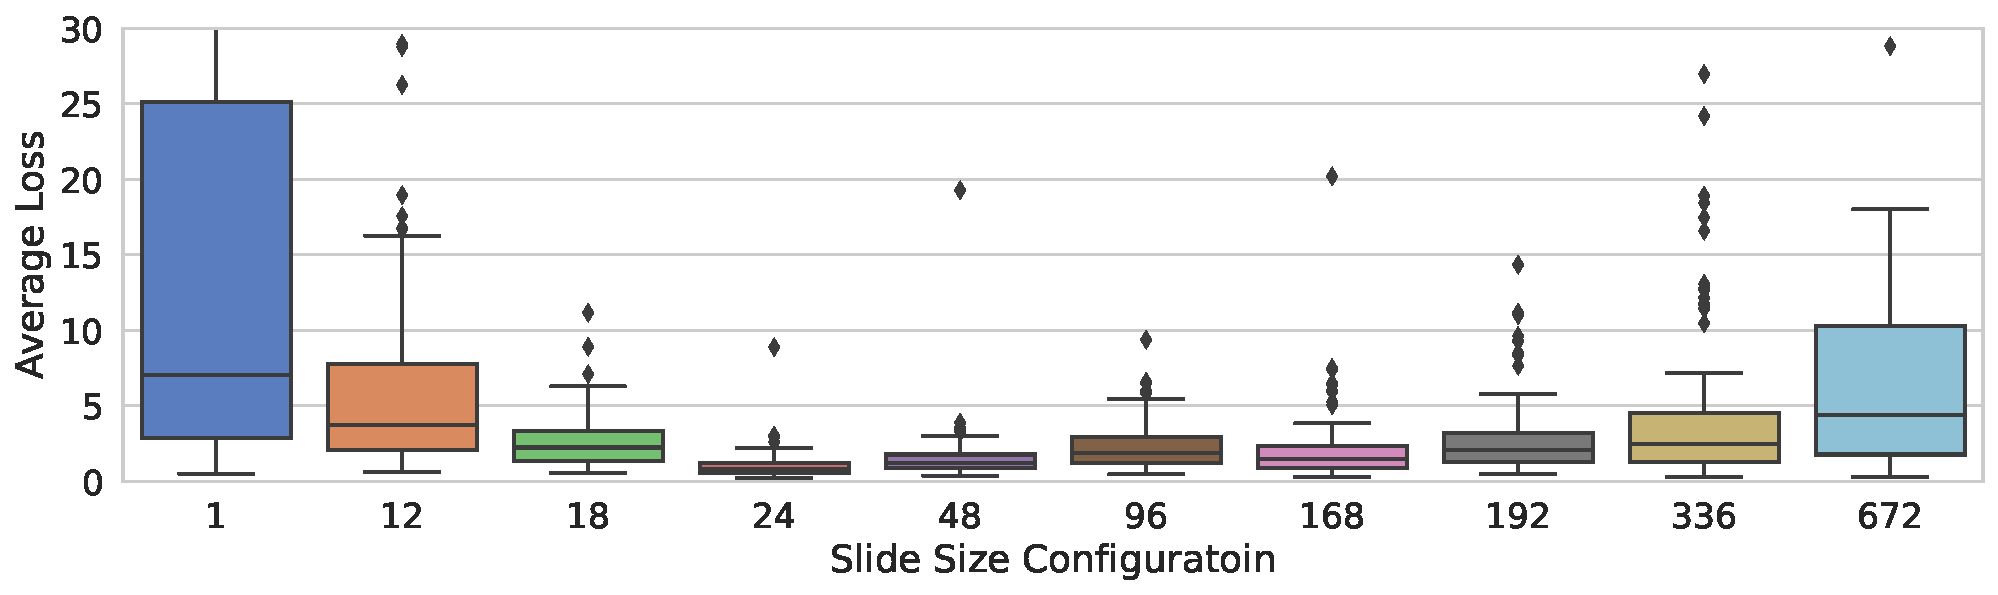
\includegraphics[width=8cm]{ralf/figures/stl_sim_fifo.pdf}
         \caption{\textbf{FIFO Event Prioritization} }
         \label{f:stl-event-prio-fifo}
     \end{subfigure} \hfill
     \begin{subfigure}[b]{\columnwidth}
         \centering
         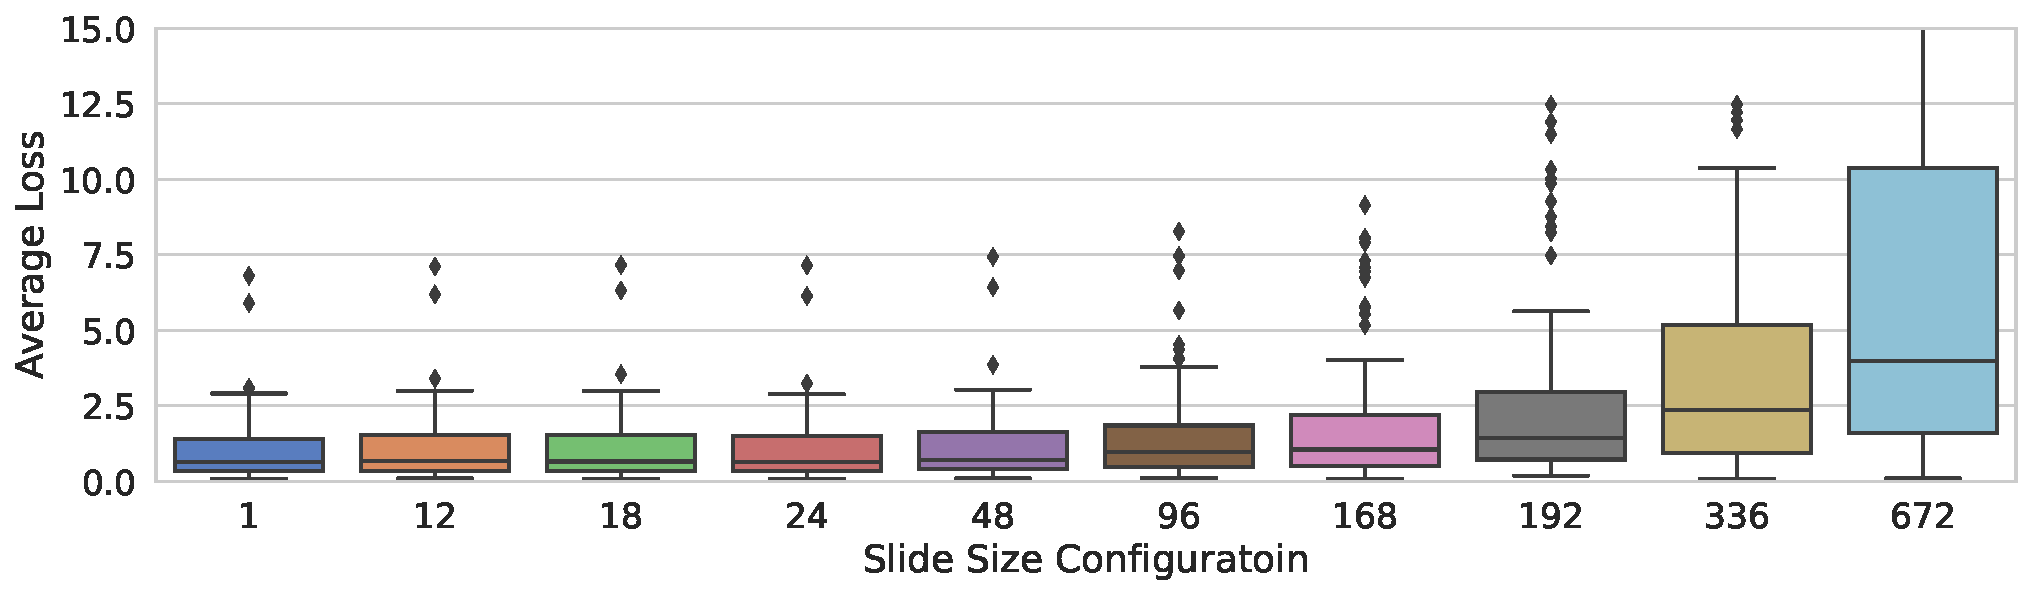
\includegraphics[width=8cm]{ralf/figures/stl_sim_lifo.pdf}
         \caption{\textbf{LIFO Event Prioritization} }
         \label{f:stl-event-prio-lifo}
     \end{subfigure}
        \caption{Distribution of average loss across key for anomaly detection workload with different window slide sizes configuration}
\end{figure}

\begin{figure}[t]
% \setlength{\belowcaptionskip}{-3pt}
% \setlength{\abovecaptionskip}{-5pt}
     \centering
     \begin{subfigure}[b]{0.5\textwidth}
         \centering
         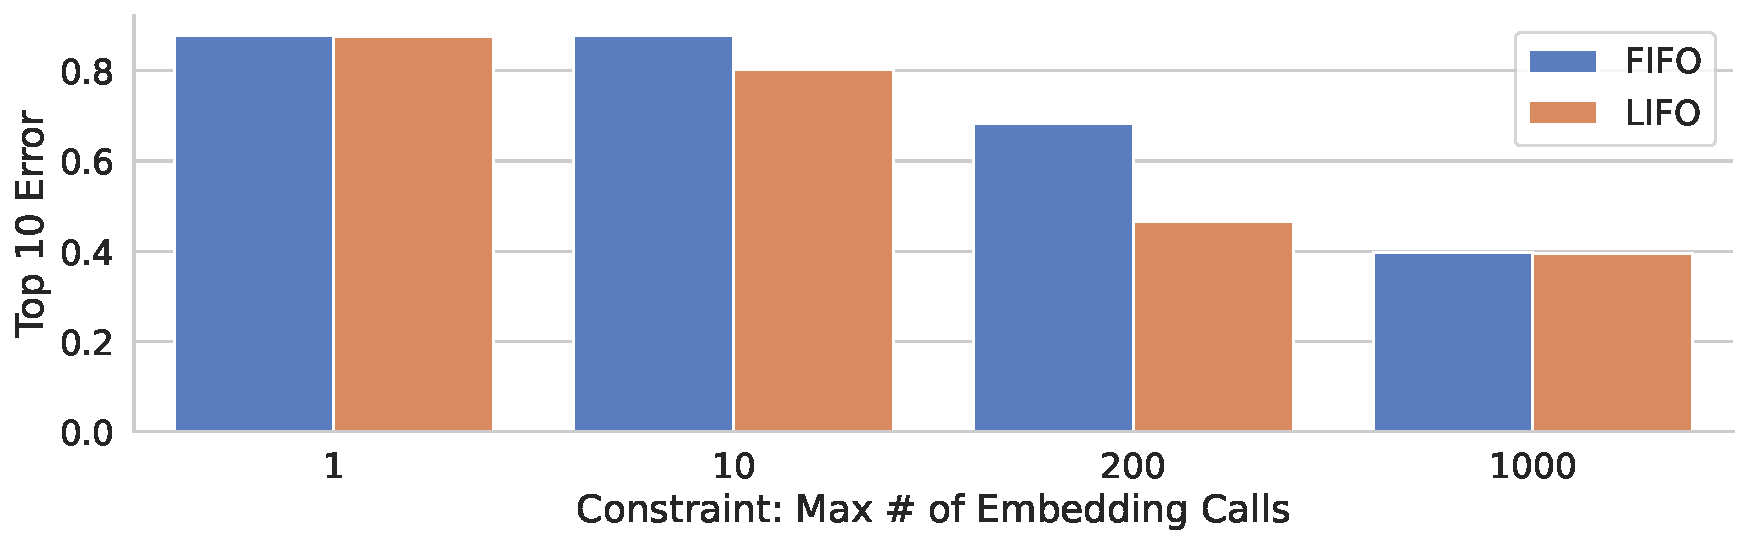
\includegraphics[width=8cm]{ralf/figures/fifo_lifo_wiki_simulation.pdf}
         \caption{\textbf{Event Prioritization}}
         \label{fig:wiki-event-sim}
     \end{subfigure} % \hfill
     \begin{subfigure}[b]{0.5\textwidth}
         \centering
         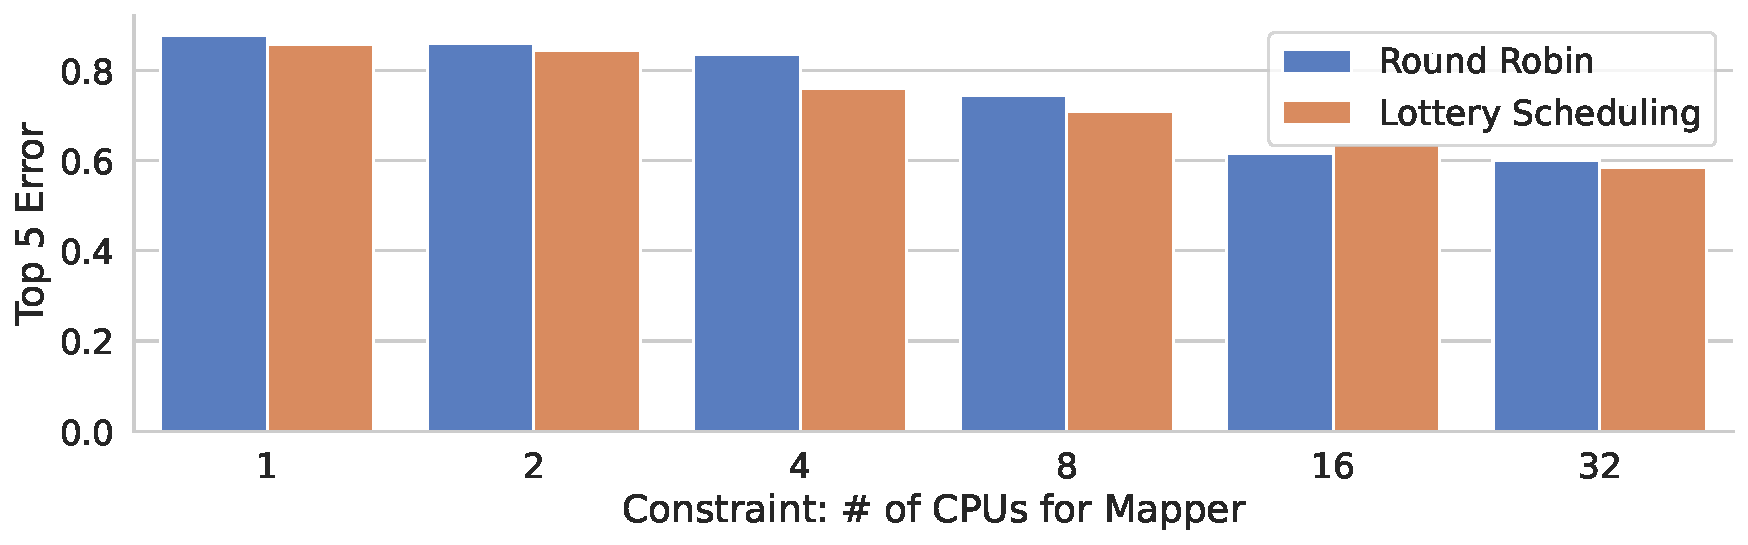
\includegraphics[width=8cm]{ralf/figures/weighted_wiki_simiulation.pdf}
         \caption{\textbf{Key Prioritization}}
         \label{fig:wiki-key-sim}
     \end{subfigure}
        \caption{Simulated results for information retrieval workload for constraints on the number of feature computations per second. \textbf{(a)} LIFO key prioritization policy outperforms FIFO policy. \textbf{(b)} The lottery scheduling policy outperforms round robin baseline.
        % We plot the downstream accuracy metrics \textbf{(a)} for policy configurations for document embeddings and the distribution of key-scores \textbf{(b)} assigned under different LP configurations. 
        %\joey{This caption doesn't match what is in the figures and also we should iterate the takeaway here as well.}
        }
    %  \begin{subfigure}[b]{0.3\textwidth}
    %      \centering
    %      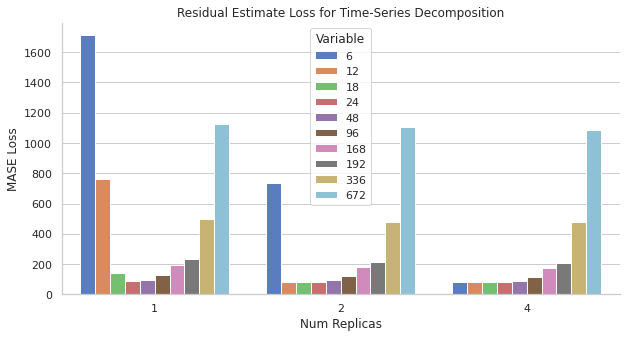
\includegraphics[width=6cm]{ralf/figures/baseline_stl_replica.png}
    %      \caption{Downstream accuracy metrics for policy configurations for time-series decomposition.}
    %      \label{fig:wiki-sim}
    %  \end{subfigure} \hfill
    %  \begin{subfigure}[b]{0.4\textwidth}
    
    % NOTE(SIMON): why is this figure a sub figure???
         \centering
         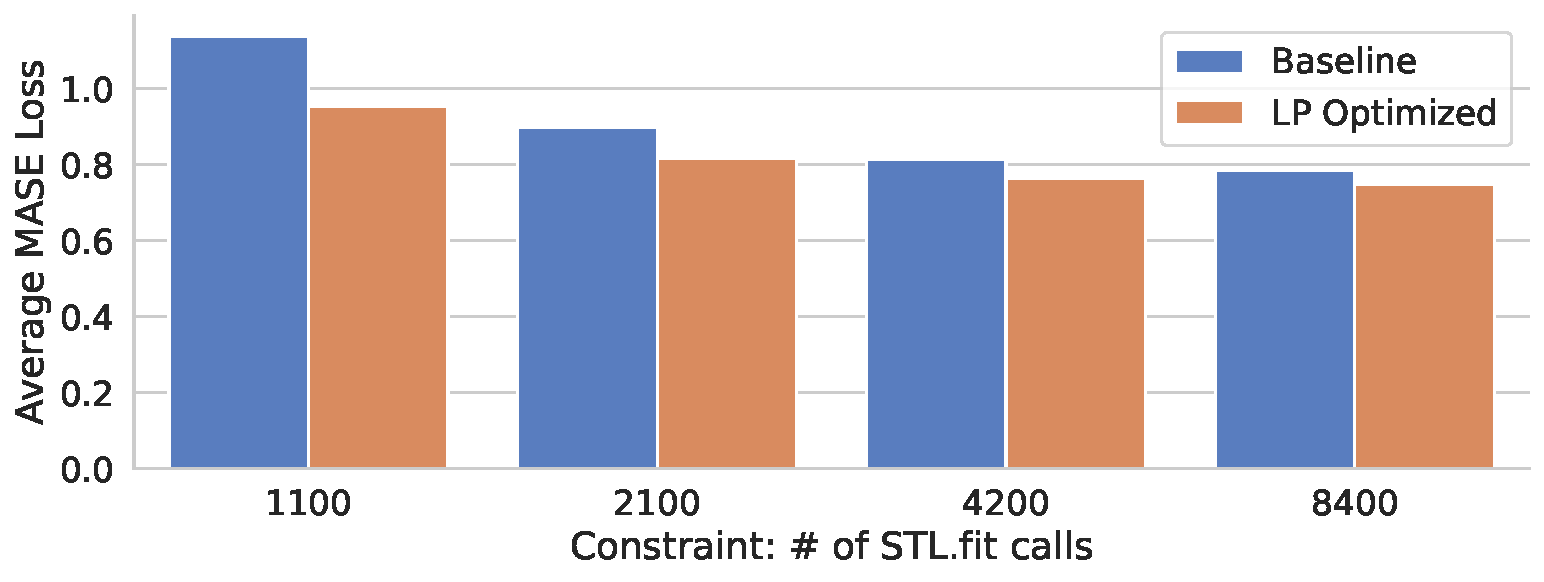
\includegraphics[width=8cm]{ralf/figures/policy_stl_cost.pdf}
        %  \caption{Distribution of key-scores assigned under different LP configurations.}
         \label{fig:stl-key-sim}
    %  \end{subfigure}
        \caption{Simulated results for anomaly detection workload. The baseline was chosen by picking the best static window slide size configuration for all the keys (e.g. slide 64 for all keys). The LP optimized plan chooses a slide size for each key and optimizes the feature store loss given the cost constraints to compute an optimal feature maintenance policy.  We see that solving the feature maintenance problem in low resource regimes translates to a significant reduction in the feature store loss.}
\end{figure}

\subsection{Simulator Experiments}
Evaluating feature maintenance policies is complicated by details of the underlying system so we begin with evaluating policy configurations for different cost constraints with the simulator described in \cref{s:planner}.  For simulations, we specify a cost constraint $C$ which specified the number of feature updates which can be performed the simulation time interval. We evaluate how changing the policy configurations affects downstream task performance of different constraints $C$.

For each workload, we explore feature maintenance policy configurations for event prioritization (performed in per-key event queues) and key prioritization (performed at the operator-level), which are summarized in \cref{table:workloads}.
% \cref{table:workloads} contains the possible configurations for each workload.
% The scheduling policies and parameter options for each workload are show in \cref{table:workloads}. 

%We use simulations to explore parameters and perform initial evaluation of our policy. We implement a system simulator which plays updates to determine what data the feature value at a given timestep was computed from. Using the generated plan, we run evaluation by determining the prediction accuracy of the prediction querying the feature store over time. We use the simulation results exploring different scheduling parameters to choose per-key parameters, which can be plugged into the simulator to adjust the scheduling policy. 

%We implement lottery scheduling to process feature updates. Lottery scheduling can be used to prioritize some events over others

\subsubsection{Event Prioritization}
For per-key event prioritization, we use two option for the parameter: FIFO and LIFO prioritization based off the event processing time.

We find that LIFO prioritization policies consistently outperform FIFO, as for both workloads new updates override any prior existing updates in-queue for the same key. For high-rates of updates, FIFO can run the danger of overfilling queues. We plot the distributed of log-loss for keys the time-series features for FIFO event prioritization in \cref{f:stl-event-prio-fifo} and LIFO event prioritization in \cref{f:stl-event-prio-lifo}. For FIFO prioritization, small slide sizes cause the featurization pipeline to fall behind, thereby increasing the staleness of features in the same way that larger slide sizes would. For LIFO prioritization, older windows are removed from the queue as new ones are product, so smaller slide sizes do not increase staleness. Decreasing the slide size has no effect once the system is at full capacity, as average frequency of feature re-computations is bounded by resource constraints. Similarly for the information retrieval workload, new versions of documents overrides prior versions so LIFO consistently performs better, as can be seen in \cref{fig:wiki-event-sim}.

\joey{We need to talk a bit about why we think LIFO out-performs FIFO.
We also need to discuss the role of resources. why do the differences vanish at 1 and 1000?}


%We find that LIFO eliminates the need for sub-sampling updates, as older updates will be removed from the queue. 

 %\textcolor{red}{Note: Running FIFO with bigger slide sizes is equivalent to LIFO with smaller slide sizes, since in expectation the number of times the window is re-fit for the key is the same since LIFO will build up the queue and then throw up the old windows}

\subsubsection{Key Prioritization}
For key prioritization, we evaluate results for policies where keys are assigned the same priority, and where keys are assigned priorities according to their impact on downstream accuracy. 

We use two different approaches to implementing key prioritization: lottery scheduling, and per-key slide sizes. Both policies are able to take in per-key parameters (i.e. the number of tickets for lottery scheduling, or the slide size) to configure how frequently updates for that key are processed. As described in section 3, we can measure accuracy of each key given different numbers of updates separately, and then use a solver to determine the resource allocation per-key to optimize downstream accuracy.

%For cross-key prioritization, we run the simulator under different parameter values for each key to determine their per-key accuracy for each parameter. For a given set of parameters for keys, we run the simulator to measure prediction accuracy and resource costs under different parameters. We then use an LP solver to choose the cost-minimizing parameters for each key to meet some overall accuracy threshold. The resulting plans can be seen in  Figure \cref{fig:wiki-plan} and Figure \cref{fig:stl-plan} for the document embedding and time series decomposition workloads, respectively.  We plug the parameters into the simulator to process the remaining edits, and evaluate the overall accuracy. We show the accuracy results compared to statis baselines (keys are treated the same way by the scheduler) in Figure \cref{fig:wiki-sim} and Figure \cref{fig:stl-sim} for the document embedding and time series decomposition workloads.

For the anomaly detection workload, we prioritize keys by using dynamic windowing to set different window slide-sizes for different keys. Lower slide size values will result in more updates per key. We assign key parameters (i.e. the slide size) by running the per-key accuracy for different slide sizes and the cost constraint through an LP-solver, to choose the best combination of slide sizes to maximize accuracy. We show the results for uniform versus non-uniform slide sizes in \cref{fig:stl-key-sim}. Lower resource budgets show the biggest gains with per-key configurations, while higher budgets show similar results. 
%We plot the tradeoff curve between total loss (over all keys) and the total number of feature updates done in Figure \cref{f:time-series-stalessness-loss}. 


For the information retrieval workload, we prioritize keys using lottery scheduling \cite{waldspurger1994lottery} to prioritize keys by assigning more tickets to higher priority keys. We assign key parameters to be proportional to how frequently the document is queried, based off past query data, to allocate more resources to frequently queried keys. We plot the top-10 error for the downstream retrieval task under different cost budgets for both the uniform and non-uniform lottery scheduling policies in \cref{fig:wiki-key-sim}. For lower resource budgets, the query-aware lottery scheduling policy allocates resources more effectively to keys which are queried often. As the resource budget increases, the impact of query-awareness decreases. 




 

 


%We plot the tradeoff curve between total loss (over all keys) and the total number of feature updates done in Figure \cref{f:time-series-stalessness-loss} for the time-series decomposoition workload. Per-key configuration of the scheduling policy significantly reduces the cost of achieving loss total loss values as compared to baseline scheduling policies. 








% \subsubsection{Time-series Decomposition}
% \label{ss:evaluation:time-series-decomposition}
% Time series decomposition is a common pre-processing step to many downstream tasks, such as anomaly detection or forecasting. Decomposition requires fitting an STL algorithms to sliding windows of the time series, to estimate the trend and seasonality patterns of the time series. We construct a time series decomposition featurization pipeline based off real-world workloads at Splunk. 

% \label{ss:evaluation:time-series-decomposition}
% \begin{itemize}
%     \item Constant ingest rate across keys - One event per key per second 
%     \item 1,000,000 keys (each represents a different time series) 
%     \item Downstream task: Calculate the residual (noise) for each new point in the time-series using the most recent trend and seasonality estimate for the time series. 
%     \begin{itemize}
%         \item Periodic queries - two classes: half of queries are once every minute, the other are once every 10s 
%         \item Accuracy metric: We evaluate the loss (error) of the residual estimates calculated using queried decomposition results. 
%         \item Ground truth: We compare the residual estimate to a residual estimate made with a model fit on the entirety of the date, which is the best estimate of the residual 
%     \end{itemize}
% \end{itemize}

% \subsubsection{Wikipedia Edit Stream}
% Embedding are often cached in feature stores. We construct a workload maintaining language model embeddings for documents which are edited over time. We use publicly available Wikipedia edit streams and page-view statistics to create representative edit and query streams. 
% \label{ss:evaluation:wikipeida}
% \begin{itemize}
%     \item Variable ingest rate accross keys  (based off recent edits stream) 
%     \item 10,000 keys (each key is for an article)
%     \item Downstream task: Rank the relevance of passages within a document to a question 
%     \begin{itemize}
%         \item Variable query pattern based off daily pageview data - distribution changes day to day 
%         \item Accuracy metric: Rank-loss of the ranking using the current embeddings 
%         \item Ground truth: Ranking of the passages with embeddings which include all updates 
%     \end{itemize}
% \end{itemize}




\subsection{System Experiments}
\label{ss:evaluation:results}
We evaluate the performance of feature maintenance policy parameters by implementing the anomaly detection workload in \system{}. We run experiment with both baseline and configured policy parameters to evaluate our feature maintenance policies. Unlike the simulation experiment, our system experiments characterize resource cost as the number of replicas available to the system, rather than the number of featurization updates. 

We consider \textit{baseline} configurations to be configurations where the same window slide size is used for each key. The LP-optimized configuration uses the per-key slide-sizes chosen from \ref{table:workloads} by the offline planner. 

%We run \system{} with a varying number of replicas to observe feature quality under varying resource constraints. We show the loss results for \cref{f:stl-real-ralf}. 

\subsubsection{Event Prioritization}
As in the simulated experiments, we run FIFO and LIFO event prioritization for the per-key queues under different slide size configurations. We show results in   \cref{f:stl-real-event-ralf}. For smaller numbers of mappers (i.e. fewer resources), LIFO performs significantly better than FIFO just as in the simulated results. 

\subsubsection{Key Prioritization}
We also implement key-prioritization in \system{} by setting per-key slide sizes with the policy configuration. Adjusting the slide-size per key allows resources to be allocated to higher-variance time-series which are more likely to benefit from frequent feature re-computations. We compare the configured policy results with baseline static slide size results in \cref{f:stl-real-ralf}. The total loss for \system{} configured by the offline planner consistently outperforms static slide size baselines for various slide sizes. 

%For our baseline, we run the pipeline with a set re-computation frequency across all keys over time. We then re-run the same pipeline with policy parameters determined by the offline solver. %\textcolor{red}{(TODO: extend time series so we don't simulate with the same data with fit the LP with)}


% \subsubsection{System Comparison: Timely Dataflow}
% We implement a prototype featurization pipeline in Timely dataflow to show our techniques are generally portable.

% We run the same experiment with multiple numbers of shards on Timely dataflow using static and configured key parameters. We show our results in \cref{f:stl-real-timely}. 

\begin{figure}[t]
\setlength{\belowcaptionskip}{-5pt}
% \setlength{\abovecaptionskip}{-5pt}
\begin{center}
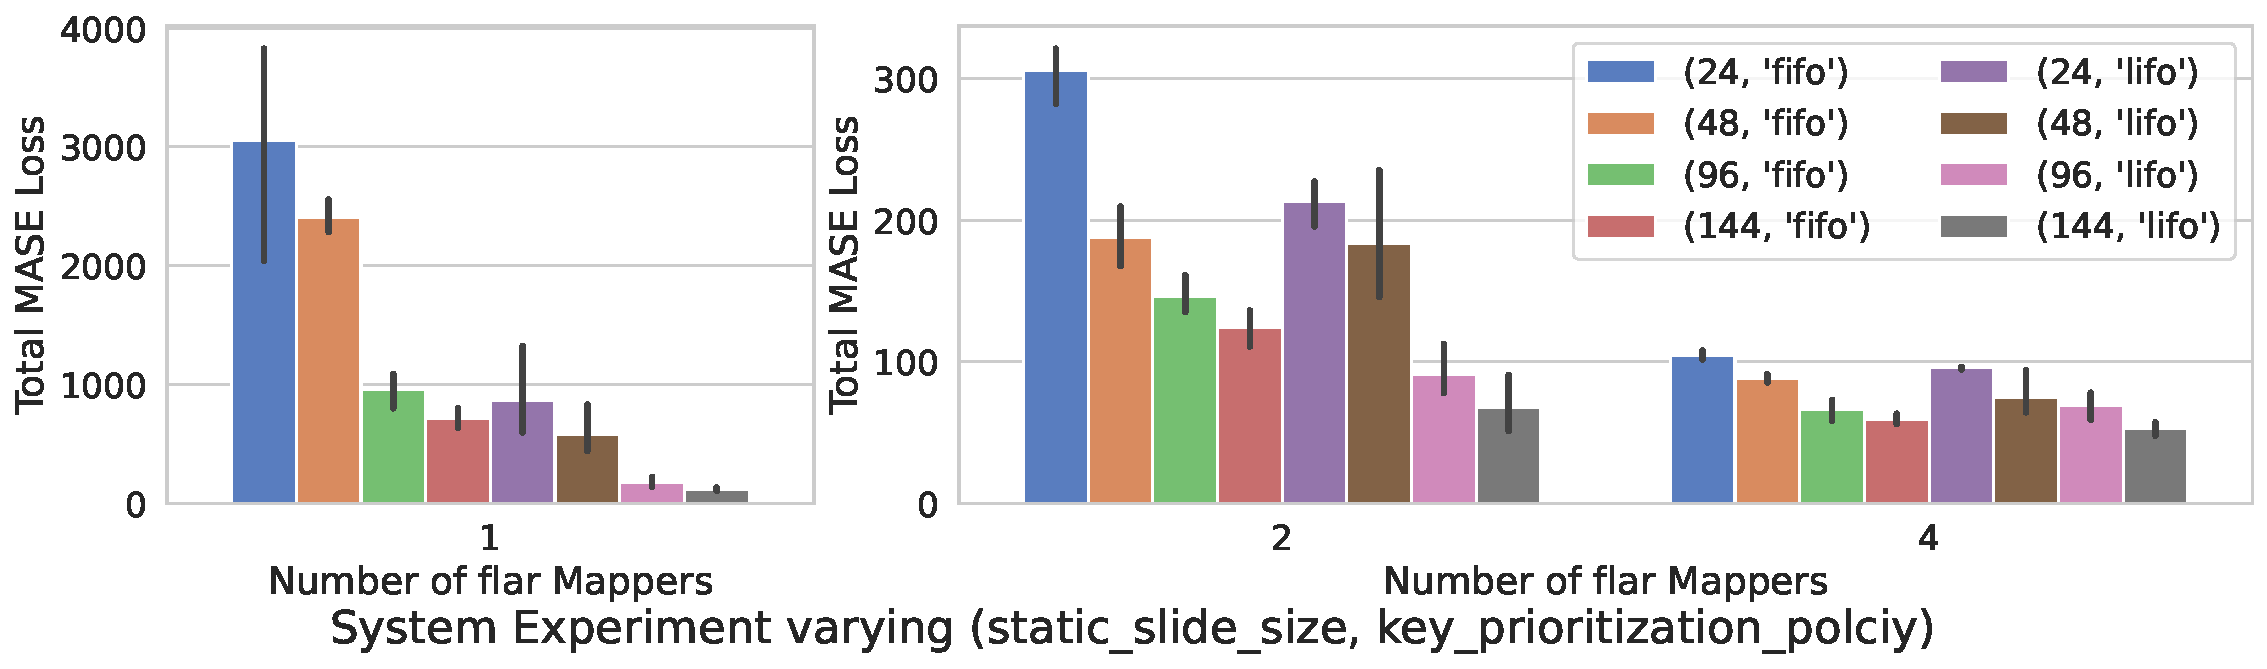
\includegraphics[width=8cm]{ralf/figures/STL_ralf_event_prioritization.pdf}
\centering
\end{center}
%     reduction_perc = (fifo_loss - lifo_loss)/fifo_loss
% (mappers, slide) reduction_perc 
% (1, 24) 0.7172083269825937
% (1, 48) 0.7598605412211124
% (1, 96) 0.8113894725242868
% (1, 144) 0.8312710950189043
% (2, 24) 0.30207810083099873
% (2, 48) 0.020346461560271093
% (2, 96) 0.37751290390956926
% (2, 144) 0.4526847180520744
% (4, 24) 0.08164146860088016
% (4, 48) 0.15641357014336177
% (4, 96) -0.05179793275749648
% (4, 144) 0.11415347558410471
\caption{FIFO vs. LIFO event prioritization for STL on \system{}. We demonstrate that LIFO key prioritization policy can improve total loss up to 83\%. }
    \label{f:stl-real-event-ralf}
\end{figure}

% %% %---------------------------
% %---------------------------
\begin{figure}[t]
\begin{center}
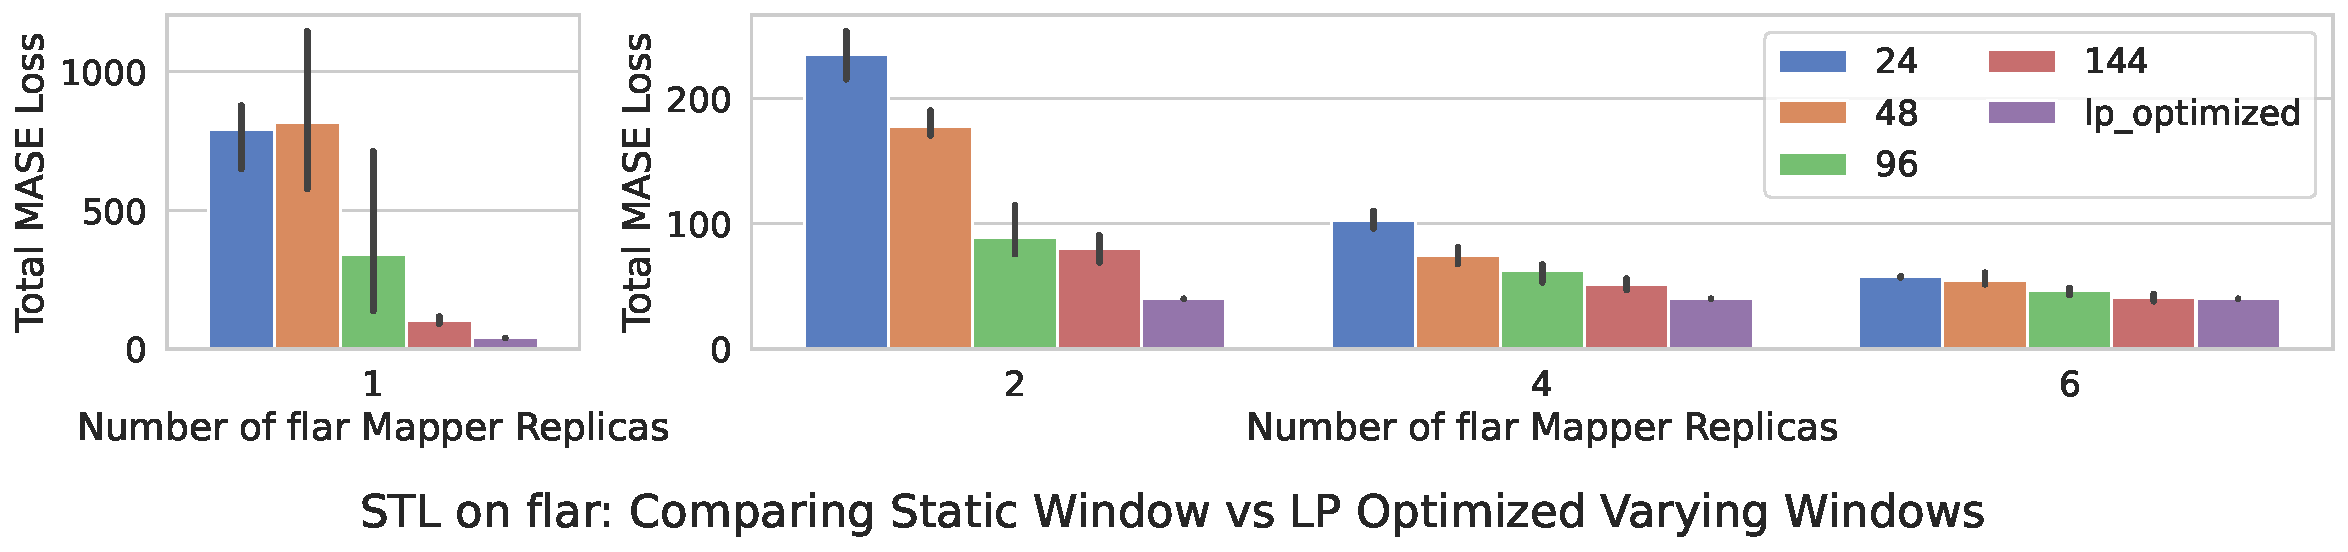
\includegraphics[width=8cm]{ralf/figures/real_stl.pdf}

\centering
\end{center}
% num_mapper, best_reduction_perc
% 1 0.15695887489846344
% 2 0.23727390017311298
% 4 0.19484476961157518
% 6 0.030014505705423924

\caption{ Static vs. dynamic (determined by the numeric solver) sliding windows on different numbers of replicas on \system{}. The optimized plan reduce loss from 3\% to 23\% depending on the resource constraint.}
    \label{f:stl-real-ralf}
\end{figure}

% \begin{figure}[t]
% \begin{center}
% \includegraphics[width=8cm]{ralf/figures/TIMELY_PLACEHOLDER.png}
% \centering
% \end{center}
% \caption{ \textcolor{red}{(TODO: this is a placeholder - numbers getting fixed)}Loss metrics for statis vs. dynamic windows with Timely Dataflow on different numbers of replicas. }
%     \label{f:stl-real-timely}
% \end{figure}



% % %---------------------------
% \begin{figure}[t]
% \begin{center}
% 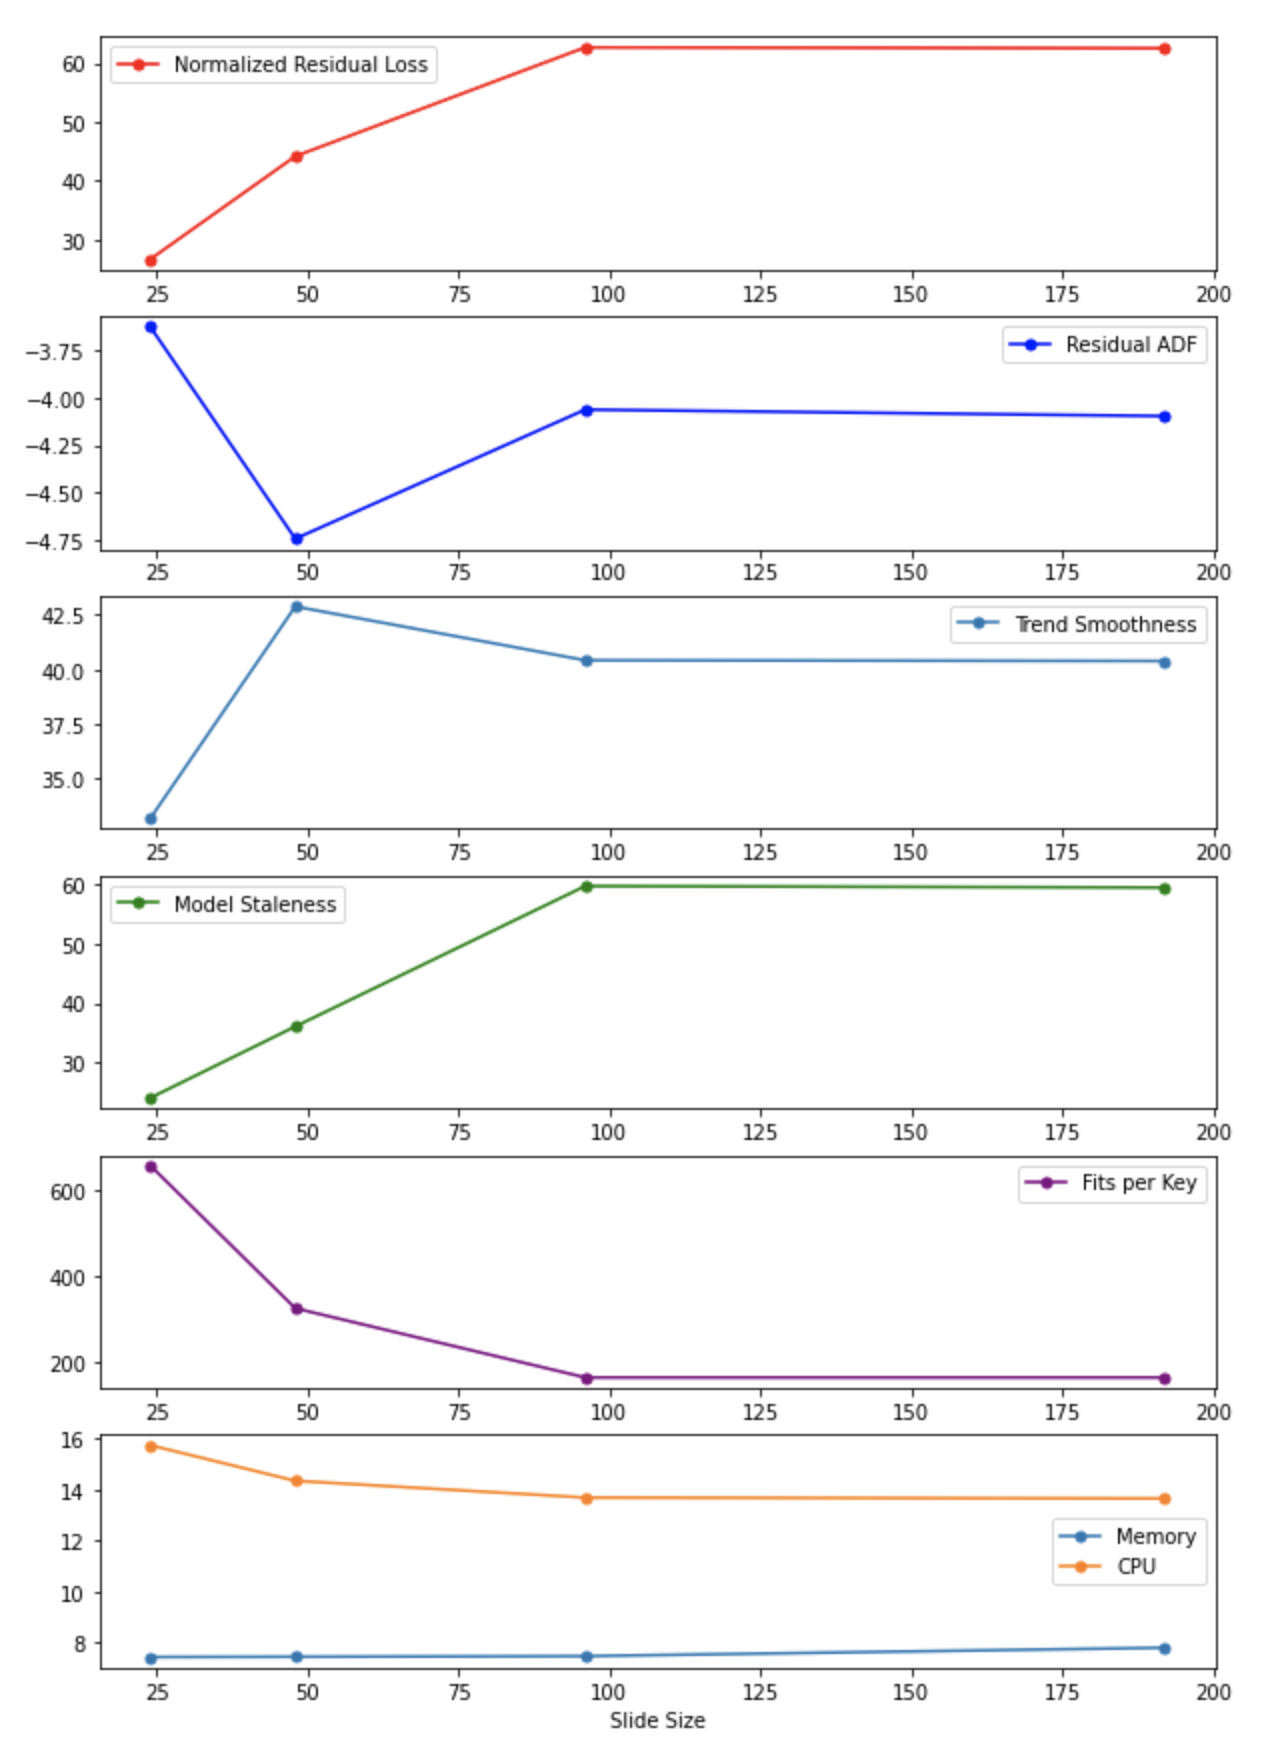
\includegraphics[width=8cm]{ralf/figures/splunk_initial.png}
% \centering
% \end{center}
% \caption{\label{fig:vectors} System and performance metrics for Time-series Decomposition workload. }
%     \label{f:time-series-decomposition-performance}
% \end{figure}

% %% %---------------------------
% %---------------------------

% %% %---------------------------
% %---------------------------
% \begin{figure}[t]
% \begin{center}
% 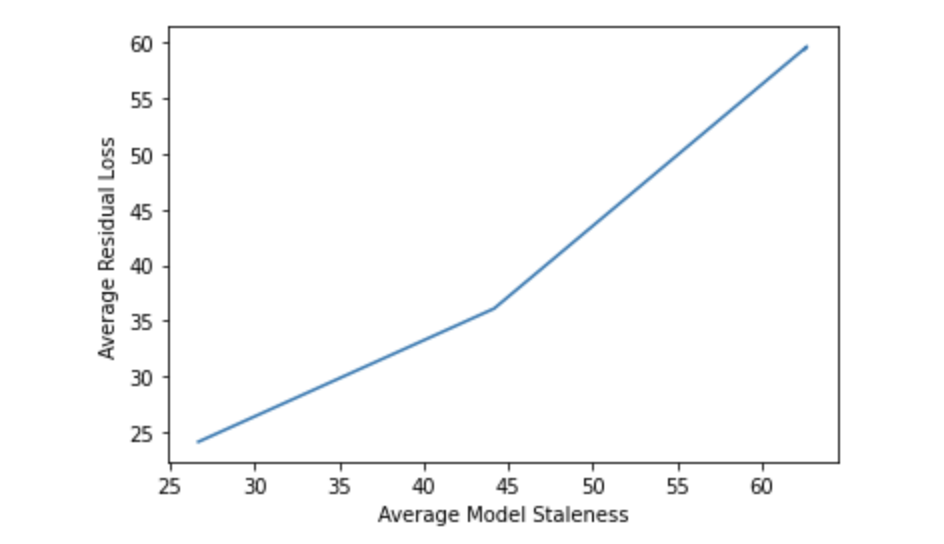
\includegraphics[width=8cm]{ralf/figures/staleness_vs_loss.png}
% \centering
% \end{center}
% \caption{\label{fig:vectors} Staleness-accuracy curve for Time-series Decomposition workload.}
%     \label{f:time-series-stalessness-loss}
% \end{figure}


% % %% %---------------------------
% % %---------------------------
% \begin{figure}[t]
% \begin{center}
% 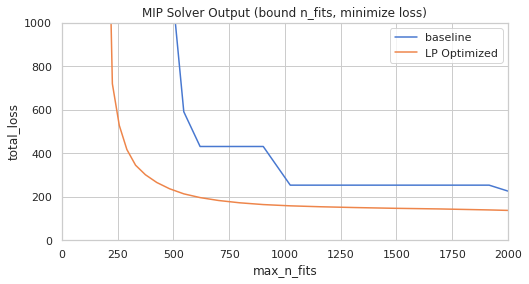
\includegraphics[width=8cm]{ralf/figures/baseline_loss.png}
% \centering
% \end{center}
% \caption{\label{fig:vectors} Baseline versus LP-optimized scheduler cost-accuracy curves.\textcolor{red}{We need one more curve - which is using past data on new data. "Baseline" also needs a new name. }}
%     \label{f:time-series-stalessness-loss}
% \end{figure}
